\documentclass[11pt]{article}

\usepackage[scale=1]{ccicons}
\usepackage{metalogo}
\usepackage{xcolor,colortbl}
\usepackage{multicol,multirow,booktabs}
\usepackage{graphicx}
\usepackage{bm}
\usepackage{fontawesome5}
\usepackage{xsim}
% Definir un nuevo tipo de ejercicio llamado "Pregunta"
\DeclareExerciseType{pregunta}{
  exercise-env = pregunta,
  solution-env = respuesta,
  exercise-name = Pregunta,
  solution-name = Respuesta,
  exercise-template = simple,
  solution-template = simple,
}

\usepackage[paper=a4paper, headheight=110pt,showframe=false, 
            layoutvoffset=2em,
            bottom=2cm, top=3.5cm, left=2.5cm, right=2.0cm]{geometry}
\usepackage[spanish, es-nodecimaldot]{babel}
\DeclareExerciseTranslations{exercise}{
  Fallback = exercise,
  English = exercise,
  Spanish = ejercicio
}
\usepackage{hyperref}
\usepackage{amsmath}
\usepackage{mismath}
\usepackage{gensymb,amssymb}
\setlength{\parindent}{3em}
\setlength{\parskip}{1em} 
\usepackage[shortlabels]{enumitem}
\usepackage{subcaption}
\usepackage{wrapfig}
\usepackage{siunitx}
%\usepackage{mathspec}
%\usepackage{unicode-math}


% Fonts can be customized here.
\defaultfontfeatures{Mapping=tex-text}
\setmainfont [Ligatures={Common}]{Linux Libertine O}
\setmonofont[Scale=0.9]{Linux Libertine Mono O}
%\usepackage[svgnames]{xcolor} % Gestión de colores
\usepackage{hyperref}
\hypersetup{
  colorlinks=true, linktocpage=true, pdfstartpage=3, pdfstartview=FitV,%
  breaklinks=true, pageanchor=true,%
  pdfpagemode=UseNone, %
  plainpages=false, bookmarksnumbered, bookmarksopen=true, bookmarksopenlevel=1,%
  hypertexnames=true, pdfhighlight=/O,%nesting=true,%frenchlinks,%
  urlcolor=Maroon, linkcolor=RoyalBlue, citecolor=Blue, %pagecolor=RoyalBlue,%
  pdftitle={},%
  pdfauthor={\textcopyright\ C. Manuel Carlevaro},%
  pdfsubject={},%
  pdfkeywords={},%
  pdfcreator={XeLaTeX},%
  pdfproducer={XeLaTeX}%
}

%% Operadores
\DeclareMathOperator{\sen}{sen}
\DeclareMathOperator{\senc}{senc}
\DeclareMathOperator{\sign}{sign}
\newcommand{\T}[1]{\underline{\bm{#1}}}
\DeclareMathOperator{\Tr}{Tr}
%\NewDocumentCommand{\evalat}{sO{\big}mm}{%
  %\IfBooleanTF{#1}
   %{\mleft. #3 \mright|_{#4}}
   %{#3#2|_{#4}}%
%}


\title{Introducción a las matemáticas}
\author{Manuel Carlevaro}
\date{Universidad de Navarra}


\begin{document}
%\maketitle

\begin{center}
\framebox[1.0\textwidth][c]{
\huge{\textsc{Introducción a las matemáticas}} 
}
\end{center} 

\begin{center}
\vspace{1em}
\Large{\textsc{Universidad de Navarra}} 
\end{center}

 \vspace{1em}

\begin{center}
\begin{tabular}{r l}
 \textbf{Tema:} & Conjuntos numéricos. \\
 \textbf{Profesor:} & Manuel Carlevaro \\
\end{tabular}\end{center}

\vspace{2em}
\section*{Actividad 1: conjuntos, pertenencia e inclusión.}

En la siguiente actividad se repasarán las definiciones y los símbolos presentados en las secciones: definición por comprensión, definición por extensión, inclusión de conjuntos, subconjuntos, pertenencia y diagramas de Venn.

\begin{exercise}
Considerar los siguientes conjuntos y completar con $\in$ o $\notin$:
\begin{enumerate}[a)]
    \item El conjunto $A$ está formado por: perro, gato, caballo, vaca y pato. \\[1.0em]
        vaca\blank{blank}$A$, elefante\blank{}$A$, tigre\blank{}$A$, caballo\blank{}$A$, perro\blank{}$A$.
    \item El conjunto $B$ está formado por países de Europa: \\[1.0em]
        Grecia\blank{}$B$, Burkina Faso\blank{}$B$, Italia\blank{}$B$, Portugal\blank{}$B$, Brasil\blank{}$B$. 
\end{enumerate}
\end{exercise}

\begin{exercise}
El conjunto $N$ está formado por las notas musicales. Representarlo por extensión y por comprensión.
\begin{enumerate}[a)]
    \item Por extensión: \blank[width=10cm]{}
    \item Por comprensión: \blank[width=10cm]{}
\end{enumerate}
\end{exercise}

\begin{exercise}
Considerar los conjuntos $A$, $B$ y $C$ que se representan a continuación en un diagrama de Venn. 
\begin{minipage}{0.45\textwidth}
\begin{enumerate}[a)]
    \item Representar los conjuntos por extensión:\\[0.5em]
        $A$: \blank[width=4cm]{} \\[0.5em]
        $B$: \blank[width=4cm]{} \\[0.5em]
        $C$: \blank[width=4cm]{} 
    \item Completar con $\subseteq$ o $\nsubseteq$ según corresponda: \\[0.5em]
        $B$ \blank{} $A$, $C$ \blank{} $A$, $C$ \blank{} $B$.
\end{enumerate}

\end{minipage}
\hfill
\begin{minipage}{0.45\textwidth}
    \begin{center}
        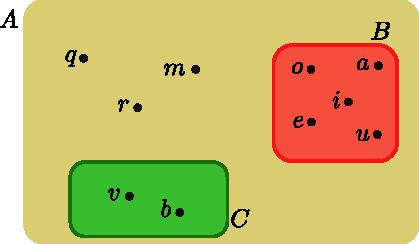
\includegraphics[width=1.0\textwidth]{figs/ej-01.pdf}
    \end{center}
\end{minipage}
\end{exercise}

\begin{exercise}
Considerar $A$, $B$ y $C$ los conjuntos definidos por comprensión de la siguiente manera:
\begin{align*}
    A &= \{\text{letras de la palabra ``vacaciones''} \} \\
    B &= \{\text{letras de la palabra ``canciones''} \} \\
    C &= \{\text{letras de la palabra ``oraciones''} \} 
\end{align*}
\begin{enumerate}[a)]
    \item Escribir por extensión los conjuntos $A$, $B$ y $C$.
    \item Decidir si se cumplen algunas de las siguientes inclusiones. En caso negativo, explicar por qué.
        \begin{multicols}{4}
        \begin{enumerate}[i)]
            \item $B \subseteq A$
            \item $B \subseteq C$
            \item $C \subseteq B$
            \item $C \subseteq A$
        \end{enumerate}
    \end{multicols}
\item Realizar un diagrama de Venn que represente los conjuntos $a$, $B$ y $C$.
\end{enumerate}
\end{exercise}

\begin{exercise}
    Escribir por comprensión al conjunto $E = \{$c, o, n, j, u, n, t$\}$. Dar tres ejemplos de subconjuntos de $E$.
\end{exercise}

\begin{exercise}
Completar con $\subseteq$ o $\nsubseteq$ según el diagrama de Venn presentado.

\begin{minipage}{0.4\textwidth}
\begin{align*}
    &A \blank{} B &B \blank{} C\\
    &C \blank{} A &C \blank{} B\\
    &B \blank{} A &B \blank{} D\\
    &D \blank{} A &C \blank{} D
\end{align*}
\end{minipage}
\hfill
\begin{minipage}{0.5\textwidth}
    \begin{center}
        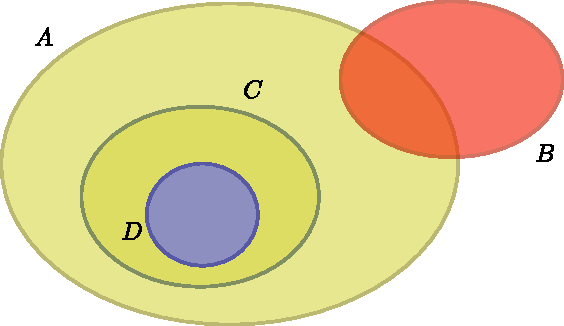
\includegraphics[width=0.9\textwidth]{figs/ej-02.pdf}
    \end{center}
\end{minipage}
\end{exercise}

\begin{exercise}
    Considerar los conjuntos $F = \{1, 2, 3, 4, 5\}$, $G = \{2, 4\}$ y $H = \{2, 4, 6\}$.
    \begin{enumerate}[a)]
        \item Decidir si las siguientes afirmaciones son verdaderas o falsas:
            \begin{multicols}{3}
                \begin{enumerate}[i)]
                    \item $2 \in F$
                    \item $4 \notin H$
                    \item $F \subseteq G$
                    \item $G \subseteq F$
                    \item $\{1, 3\} \subseteq F$
                    \item $H \nsubseteq G$
                \end{enumerate}
            \end{multicols}
        \item Realizar un diagrama de Venn que represente a los conjuntos $f$, $G$ y $H$.
    \end{enumerate}
\end{exercise}

\section*{Actividad 2: operaciones con conjuntos.}

\begin{exercise}
    Considerar los conjuntos $A = \{a, b, c, d, e\}$, $B = \{a, b, c\}$ y $C = \{d, e, f, g\}$. Calcular los siguientes conjuntos:
    \begin{multicols}{6}
        \begin{enumerate}[a)]
            \item $A \cup B$
            \item $A \cap B$
            \item $A - B$
            \item $B - A$
            \item $A \cup C$
            \item $A\cap B \cap C$
        \end{enumerate}
    \end{multicols}
\end{exercise}

\begin{exercise}
En cada caso, sombrear la región del diagrama de Venn que le corresponde a cada operación.
\begin{multicols}{3}
    \begin{enumerate}[a)]
        \item $A \cup B$ \\
            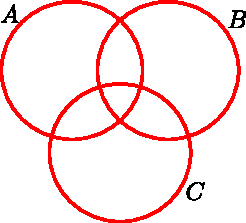
\includegraphics[scale=0.7]{figs/fig-07.pdf}
        \item $A \cap B$ \\
            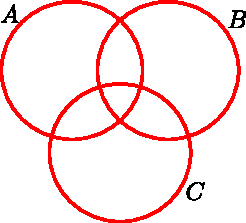
\includegraphics[scale=0.7]{figs/fig-07.pdf}
        \item $C - B$\\
            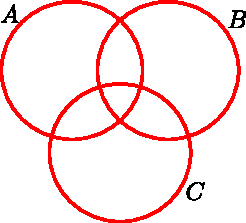
\includegraphics[scale=0.7]{figs/fig-07.pdf}
        \item $A \cup B - C$\\
            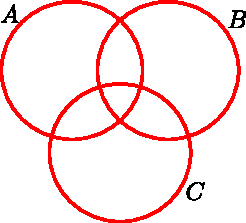
\includegraphics[scale=0.7]{figs/fig-07.pdf}
        \item $A \cup B$\\
            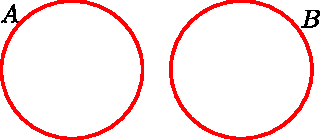
\includegraphics[scale=0.7]{figs/fig-08.pdf}
        \item $A \cap B$\\
            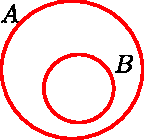
\includegraphics[scale=0.7]{figs/fig-09.pdf}
    \end{enumerate}
\end{multicols}
\end{exercise}

\begin{exercise}
Escribir la operación indicada en cada diagrama de Venn.
\begin{multicols}{2}
    \begin{enumerate}[a)]
        \item 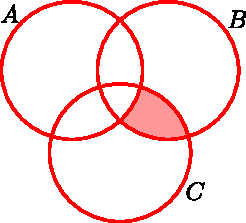
\includegraphics[scale=1.0]{figs/fig-10.pdf}
        \item 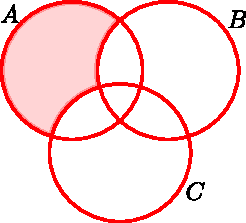
\includegraphics[scale=1.0]{figs/fig-11.pdf}
    \end{enumerate}
\end{multicols}
\end{exercise}

\begin{exercise}
En una escuela hay 75 personas que saben tocar alguno de los siguientes instrumentos musicales: flauta, guitarra o piano. Del total de personas en la escuela hay dos personas que saben tocar los tres instrumentos. Hay 15 personas que solamente saben tocar la flauta, y hay 12 personas que solamente saben tocar el piano. También hay 9 personas que saben tocar el piano y la guitarra pero no saben tocar la flauta; dos personas que solamente saben tocar el piano y la flauta pero no saben tocar la guitarra, y dos personas que saben tocar la guitarra y la flauta pero no saben tocar el piano. ¿Cuántas personas saben tocar únicamente la guitarra?
\end{exercise}


\section*{Actividad 3: conjuntos numéricos}

\begin{exercise}
En la figura del eje numérico representando los números racionales se muestra que entre dos números racionales diferentes siempre existen otros números racionales ubicados entre medio. Por ejemplo, el número $1.75$ se ubica entre los números $1.7499$ y $1.751$.
\begin{enumerate}[a)]
    \item ¿Qué otro número racional está entre el $1.75$ y el $1.7499$? ¿Y entre el $1.75$ y el $1.751$?
    \item ¿Qué otro número racional está entre el $-0.201$ y el $-0.199$? ¿Y entre el $-3.45$ y el $-3.44$?
    \item ¿Qué otro número racional puede ubicarse entre el $0.\hat{6}$ y el $0.67$?
\end{enumerate}
\end{exercise}

\begin{exercise}
Esriba cuatro elementos de cada conjunto numérico: $\mathbb{N}$, $\mathbb{Z}$, $\mathbb{Q}$, $\mathbb{I}$ y $\mathbb{R}$. 
\end{exercise}

\begin{exercise}
Señale, en los siguientes casos, a qué conjunto de número pertenecen:

$0$ \blank{}, $-10$ \blank{}, $40$ \blank{}, $\frac{22}{7}$ \blank{}, 
$\frac{21}{7}$ \blank{}, $\sqrt{7}$ \blank{}, $0.\widehat{14}$ \blank{}, 
$-\pi$ \blank{}.
\end{exercise}

\begin{exercise}
Marque, en la siguiente cuadrícula, todos los números primos.
\begin{center}
    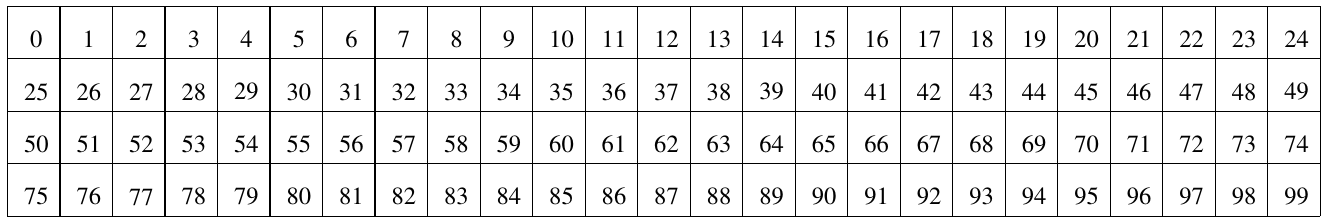
\includegraphics[width=1.0\textwidth]{figs/primos.png}
\end{center}
\end{exercise}

\begin{exercise}
Simplifique las siguientes fracciones para obtener una fracción irreducible equivalente.
\begin{multicols}{6}
    \begin{enumerate}[a)]
    \item $\frac{8}{12}$
    \item $\frac{42}{12}$
    \item $\frac{700}{100}$
    \item $\frac{16}{36}$
    \item $\frac{243}{405}$
    \item $\frac{97}{83}$
\end{enumerate}
\end{multicols}
\end{exercise}

\section*{Actividad 4: operaciones algebraicas}

\begin{exercise}
Identifique qué propiedad se está utilizando en los siguientes casos.
\begin{multicols}{2}
    \begin{enumerate}[a)]
        \item $7 + 10 = 10 + 7$
        \item $2(3+5) = (3+5)2$
        \item $(x+2y) +3z = x +(2y+3z)$
        \item $2(A+B) = 2A + 2B$
        \item $(5x+1)3 = 15x + 3$
        \item $(x+a)(x+b) = (x+a)x+(x+a)b$
    \end{enumerate}
\end{multicols}
\end{exercise}

\begin{exercise}
Escriba en cada espacio la expresión correspondiente utilizando la propiedad indicada.
\begin{enumerate}[a)]
\item Propiedad conmutativa de la suma: $x+3=$ \blank[width=3cm]{}
\item Propiedad conmutativa del producto: $(a+b) \cdot(3+c) =$ \blank[width=3cm]{}
\item Propiedad asociativa del producto: $7(3x) =$ \blank[width=3cm]{}
\item Propiedad asociativa de la suma: $(3+x+(4+y)) =$ \blank[width=3cm]{}
\item Propiedad distributiva: $4(A+B) =$ \blank[width=3cm]{}
\item Propiedad distributiva: $5x + 5y =$ \blank[width=3cm]{}
\end{enumerate}
\end{exercise}

\begin{exercise}
Utilice las pripiedades algebraicas para escribir cada expresión eliminando los paréntesis. Indique las propiedades utilizadas en casa caso.
\begin{multicols}{3}
    \begin{enumerate}[a)]
        \item $3(x+y)$
        \item $(a+b)7$
        \item $4(2m)$
        \item $(3a)(b+c+2d)$
        \item $(3+a)(5+b)$
        \item $5(a+4(x+y))$
        \item $(3+x)+5+(b+3r)$
        \item $(4(2m))x$
    \end{enumerate}
\end{multicols}
\end{exercise}

\begin{exercise}
Realice las siguientes operaciones indicando las propiedades utilizadas en cada caso.
\begin{multicols}{3}
    \begin{enumerate}[a)]
        \item \[\frac{1}{4} + \frac{1}{5} \]
        \item \[ \frac{3}{10} + \frac{4}{15} \]
        \item \[ \frac{2}{3} - \frac{3}{5} \]
        \item \[ 1 + \frac{5}{8} - \frac{1}{6} \]
        \item \[ \left(\frac{1}{2} - \frac{1}{3}\right)\left(\frac{1}{2} + \frac{1}{4}\right) \]
        \item \[ \frac{2}{\frac{2}{3}} - \frac{\frac{2}{3}}{2} \]
        \item \[ \frac{\frac{1}{12}}{\frac{1}{8} - \frac{1}{9}} \]
        \item \[ \frac{2 - \frac{3}{4}}{\frac{1}{2} - \frac{1}{3}} \]
        \item \[ \frac{3}{5} \cdot \frac{5}{13} - \frac{4}{5} \left(-\frac{12}{13}\right) \]
        \item \[ \frac{\frac{2}{5} + \frac{1}{2}}{\frac{1}{10} + \frac{3}{15}} \]
    \end{enumerate}
\end{multicols}
\end{exercise}

\begin{exercise}
    Utilice las propiedades algebraicas para escribir cada expresión eliminando los paréntesis y que quede una \textbf{única} fracción. Algunas indicaciones:
    \begin{itemize}
        \item Trabajar paso a paso, haciendo una única cuenta a la vez.
        \item Mantener la \textbf{fracción principal} al mismo nivel que el signo $=$ en cada renglón.
    \end{itemize}

\begin{multicols}{3}
\begin{enumerate}[a)]
    \item \[ \frac{4a}{7} \cdot \frac{1}{2b} \]
    \item \[ \frac{xy}{mn} \left(\frac{m}{n}\right) \]
    \item \[ \frac{2a}{3b} \div \frac{6a}{c} \]
    \item \[ \frac{2b}{3} - \frac{b}{2} + \frac{b}{4} \]
    \item \[ \frac{5a}{6} - \frac{5a}{12} - \frac{a}{3} \]
    \item \[ \frac{4}{n} + \frac{3}{n} + \frac{5}{n} \]
    \item \[ \frac{3k + 5}{5} + \frac{k+3}{3} \]
    \item \[ \frac{3k+5}{5} - \frac{k+3}{3} \]
    \item \[ \frac{2a-5}{14 a} - \frac{4-a}{7a} \]
    \item \[\frac{2}{b} + \frac{2}{c} + \frac{5}{x} \]
    \item \[ \frac{a - \frac{b}{3}}{a} \]
    \item \[ m + 4 - \frac{1}{ac} \]
    \item \[ \frac{\frac{1}{2} +1}{\frac{1}{2} - 1} \]
    \item \[ \frac{1+\frac{1}{n}}{\frac{1}{n} + \frac{1}{m}} \]
\end{enumerate}
\end{multicols}
\end{exercise}

\begin{exercise}
Evalúe cada expresión.
\begin{multicols}{5}
\begin{enumerate}[a)]
\item $-7^3$
\item $(-7)^3$
\item $(-7)^0$
\item \[ 5^2 \cdot \left(\frac{1}{5}\right)^3 \]
\item \[ \frac{10^7}{10^4} \]
\item \[ \frac{3}{3^{-2}} \]
\item \[ \frac{4^{-3}}{2^{-8}} \]
\item \[ \frac{3^{-2}}{9} \]
\item \[ \left(\frac{1}{4}\right)^{-2} \]
\item \[ \left(\frac{2}{3}\right)^{-3} \]
\item \[ \left(\frac{3}{2}\right)^{-2} \cdot \frac{9}{16} \]
\item \[ \pow{\frac{1}{2}}{4} \cdot \pow{\frac{5}{2}}{-2} \]
\end{enumerate}
\end{multicols}
\end{exercise}

\begin{exercise}
Simplifique las siguientes expresiones eliminando todos los paréntesis y todos los exponentes negativos (todos los exponentes deben quedar positivos).
\begin{multicols}{3}
\begin{enumerate}[a)]
\item \[ a^9 a^{-5} \]
\item \[ (3y^2)(4y^5) \]
\item \[ (12 x^2 y^4)\left(\frac{1}{2} x^5 y\right) \]
\item \[(6y)^3 \]
\item \[ \frac{x^9 (2x)^4}{x^3} \]
\item \[ \frac{a^{-3} b^4}{a^{-5} b^5} \]
\item \[ b^4\left(\frac{1}{3} b^2\right)(12 b^{-8}) \]
\item \[ (2s^3 t^{-1})\left(\frac{1}{4}s^6\right)(16 t^ 4) \]
\item \[ (rs)^3 (2s)^{-2}(4r)^4 \]
\item \[ (2 u^2 v^3)^3 (3u^3 v)^{-2} \]
\item \[ \frac{(x^2 y^3)^4 (xy^4)^{-3}}{x^2 y} \]
\item \[ \left(\frac{c^4 d^3}{c d^2}\right) \left(\frac{d^2}{c^3}\right)^3 \]
\end{enumerate}
\end{multicols}
\end{exercise}

\end{document}
